\documentclass{emulateapj}
%\documentclass[12pt,preprint]{aastex}

\usepackage{graphicx}
\usepackage{float}
\usepackage{amsmath}
\usepackage{epsfig, floatflt}
\usepackage{natbib, hyperref}
\usepackage{url}


\begin{document}
	
	\title{Ast3310 Project Nr. 1: Modelling a Stellar Core and Radiation Zone}
	
	\author{Nils-Ole Stutzer}
	
	%\email{nilsole2009@live.no}
	
	%\altaffiltext{1}{Institute of Theoretical Astrophysics, University of
		%Oslo, P.O.\ Box 1029 Blindern, N-0315 Oslo, Norway}
	\section*{Introduction}
	In order to understand the nature of stars, it is essential to understand how the energy produced in the stellar core propagates through the stars layers. The first step in researching the energy transport is to understand how the energy is transported by means of radiation through the extremely dense and hot inner part of the star, the so called radiation zone. This part of the star is so dense and hot that it may take the energy produced in the stellar core many thousend years to travel all the way to the stellar surface, as the mean free path of a gamma photon is very small.
	In this report we will focus on how we made a model for the stellar radiation zone using numerical simulations in Python. The final aim being to understand how different initial conditions affect the stellar core and the radiationzone, so as to find initial conditions that produce a stable stellar core and radiation zone.
	
	\section*{Methode}
	To make a model of the stellar radiation zone we need to make use of the laws of physics that govern the stellar interior. But because this is quite a complex system of coupled processes we need to make some assumptions in order to obtain a solvable task. First we assume that the radiatition zone of the star is made out of thin shells, with approximate constant density. Next we can assume that the star is in hydrostatic equilibrium. The third assumption is that all energy produced by the star comes from the fusion processes in its core. Since we are only interested in the energy transport through radiation we neglect convection. Thus the energy only diffuses through radiation. These assumpions result in the coupled differential equations
	
	\begin{align}
		\frac{\partial r}{\partial m} & = \frac{1}{4 \pi r^2 \rho}
		\label{eq:diff1}\\
		\frac{\partial P }{\partial m} & = -\frac{Gm}{4\pi r^4}
		\label{eq:diff2}\\
		\frac{\partial L }{\partial m} & = \epsilon = \sum{ Q_{ik}r_{ik}}
		\label{eq:diff3}\\
		\frac{\partial T}{\partial m} & = -\frac{3\kappa L}{256 \pi^2\sigma r^4T^3},
		\label{eq:diff4}
	\end{align}
	where the first equation comes frome the first assumption, the second comes from the second assumption etc. Here $\rho$, $m$, $L$ and $\epsilon$ denote the density, mass, luminosity and energy produced respectively, within a shell of radius $r$ and temperature $T$. $Q_{ik}$ and $r_{ik}$ are the energy produced and reaction rate of the $ik$-th fusion reaction reaction of the PP-chains (We do not consider high enough temperatures for CNO-cycle to be important). These where found by using the \text{energy\_production} class implemented as discribed in Appendix C in the lecture notes of the course. The reason the free variable is choosen to be $m$ and not $r$ is that the differential equations behave more stable if $m$ is chosen as the free variable. In addition to the four coupled differential equations we assume that we have an ideal gas
	\begin{align}
		P_G = \frac{\rho}{\mu m_u} k_B T,	
	\end{align}
	where $\mu$ is the mean molecular weight of the sun, $m_u$ is an atomic mass unit in kg and $k_B$ is the Boltzmann constant. The expression for gas pressure is only used to find the initial pressure so as to initiallize the PDE in eq. (\ref{eq:diff2}). Also the expressuion for gas pressure solved with respect to the the density $\rho$, which is used in the PDEs. In addition we have the radiation pressure $P_R = \frac{4\sigma}{3c}T^4$, where $\sigma$ is the Stefan-Boltzmann constant and $c$ is the speed of light. This gives an expression for the total pressure used to initialize the differential equation (\ref{eq:diff2}) 
	\begin{align}
		P = P_G + P_R.
		\label{eq:pressure}
	\end{align}
	The opacity in eq. (\ref{eq:diff4}) is a function of both the density $\rho$ and temperature $T$. This function is found by interpolating the data provided in the file \texttt{opacity.txt}. 
		
	Next we need to calculate the mean molecular weight $\mu$ used to calculate the density and the initial pressure. For this we assume that all the hydrogen and helium is fully ionized. Thus each hydrogen atom consists of one nucleus and one electron, and each helium atom consists of one nucleus and two electrons. They therefore contribute with two and three particles per nucleon respectively. We also assume that all the metals are fully ionized, meaning that Lithium and Beryllium contribute with four and five particles per nucleus each.
	Thus the mean molecular weight 
	\begin{align}
		\mu &= \frac{1}{\frac{2}{1}X_{^1_1\text{H}} + \frac{3}{3}Y_{^3_2\text{He}} + \frac{3}{4}Y_{^4_2\text{He}} + \frac{4}{7}Z_{^7_3 \text{Li}} + \frac{5}{7}Z_{^7_4\text{Be}} + \frac{2}{2}Z}\\
		&=\frac{1}{2X_{^1_1\text{H}} + Y_{^3_2\text{He}} + \frac{3}{4}Y_{^4_2\text{He}} + \frac{4}{7}Z_{^7_3 \text{Li}} + \frac{5}{7}Z_{^7_4\text{Be}} + Z}\\ 
		& \approx 0.614,
	\end{align}
	where the other metals $Z$ contribute with two particles and are assumes to have an averege mass of $2u$. The mass fractions $X_{^1_1\text{H}} = 0.7$, $Y_{^3_2\text{He}} = 10^{-10}$, $Y_{^4_2\text{He}} = 0.29$, $Z = 0.01$, $X_{^7_3\text{Li}} = 10^{-13}$ and $X_{^7_4\text{Be}} = 10^{-13}$. Also it is important to note that it is not all to importen to which degree the metals are ionized, because they are so rare, thus just assuming they are fully ionized is not a bad approximation.

	It is now time to take a look at how to solve the differential equations. In theory one can use any arbitrary integration algorithm, but we choose to use the Runge-Kutta order four (RK4) algorithm because it is a higher order methode with superior precision to lower order methods like Euler's methode. Meaning that the same choise of $\partial m$ using RK4 will be quite more stable then when using Eulers methode. 
	
	Further we implemented variable step length which could be turned on or off by a boolean input argument. When using a variable step length the local relative error iss held below a given tolerance. This is done by letting 
	\begin{align}
		\partial m = - \frac{pV}{|f|}, 
	\end{align}
	where $p$ is the set tolerance, $V$ is the current value of the function to integrate and $f$ is its derivative at the current value. Because we have several differential equations, we need to calcualte $\partial m$ for all of them, and then we use the one that is the smallest so as to ensure the best accuracy.
	Therefore the precision of the RK4 algorithm will then be even further improved. Also the integration may require less iterations, because the program chooses when it is resonable to use big or small steps in the integration.   
	
	After comparing the program output to the plots in the sanity check we can move on to the testing of initial values. The idea is that we change the value of each of the initial conditions, while holding the others constant. We tested with different initial radii $R_0$, temperatures $T_0$ and densities $\rho_0$. The reason we did not test different initial pressures is that the pressure is calculated using eq. (\ref{eq:pressure}) which is a function of the initial temperature $T_0$ and denity $\rho_0$. Thus testing different initial pressures is not necessary. 
	
	If we then test several different changes to each initial condition we can get a feeling how each of the changes affect the model, and which changes may compensate for others. This testing is done in several \texttt{for}-loops, where each loops through a 1/5 to 5 factor change to the initial conditions provided. These provided initial conditions are $L_0=L_\odot$, $R_0=0.72R_\odot$, $M_0 = 0.8M_\odot$, $\rho_0 = 5.1\overline{\rho}_\odot$ and $T_0 = 5.7\cdot10^{6}$ K, which are the initial conditions of the bottom of the convection zone. The different solutions are then ploted next to each other so as to see how the changes to the initial conditions change the simulations. Also after getting a feeling for the behaviour of the different changes one can then explore how one change in a initial condition may affect another variable, and how yet another initial value can compensate for that change. For instance it should be expected that the pressure will be strongly dependent on changes on the temperature and density, because the pressure is proportional to both quantities through the equation of state.  
	
	Having experimented with different initial values we are ready to try to find a model of a star where both the radius and luminocity go to zero when the mass goes to zero (within a $\pm5$\% tolerance of their initial values). This can be done in a simple trial and error strategy, where the knowledge achieved for how the change in different initial values changes the outcome of the simulations. 
	
	Another approach, which we chose, is to use the knowledge obtained by experimenting with different initial values and then loop over a grid of different initial values for which there was a sigificant change observed in the resulting solution. More specifically we chose to loop over the two quantities that seemed to have the greatest effect on the simulation outcome. These where found to be the initial denity and radius. Further if this strategy would not provide a stable star, one could add another loop, over for instance the temperature, to further test for more stable solutions to the simulations. The last elements of the radius, luminocity and mass arrays produced by the looped over initial values were added to their respective matrix. Also in each of the iterations the luminocity and mass values added to their matrices were divided by $L_\odot$ and $M_\odot$, while the radius values were divided by the current looped over radial initial condition. These three matrices, representing grid of tested initial values, can due to their dimensionless form be added together into a combined matrix. Because it is a solution where the luminocity and radius goes towards zero when the mass approaches zero, we simply need to find where the added dimensionless values $L_\text{last}/L_\odot + R_\text{last}(R_\text{init})/R_\text{init} + M_\text{last}/M_\odot$ approach zero (within the 5\% tolerance) go towards zero. Here init denotes the current initial value and last denotes the current last array value found in each loop iteration. Because we break the integration loop that solved the PDEs when the mass is negative, the luminocity and the radius should always be positive. Thus the most stable star we obtain must be the one where the combined matrix $L_\text{last}/L_\odot + R_\text{last}(R_\text{init})/R_\text{init} + M_\text{last}/M_\odot$ is at its minimum. The initial values for this best model will then simply be the grid coordinates in the matrix.
	
	The best model found can then be used to plot the values for $T$, $L$, $\epsilon$, $\rho$, $P$ and $m$ as a function of the radius $r$. These plots will then give a view of how the different quantities change over the stars profile.  
	
	\section*{Results/Discussion}
	Each time a section of the program was finished we compared their outputs to the provided sanity checks. Generally all the sanity checks were passed without any significant errors. Comparing the $\kappa$ data provided to the interpolated once, a small diviation in the second desimal of $\log_{10}\kappa$ was observed, but rounding up the same values as in the table were achieved. Also when comparing the plots made by the program to the provided plots, there was basically no difference one could see with the bare eye. When trying to calculate the pressure $P$ as a function of $\rho$, we got the input density $\rho$ back when calling the density function with the argument $P(\rho)$. Thus we can draw the conclusion that the density and pressure functions work fine, and since the other sanity checks went good we conclude that the program is ready for use.
	\begin{figure*}
		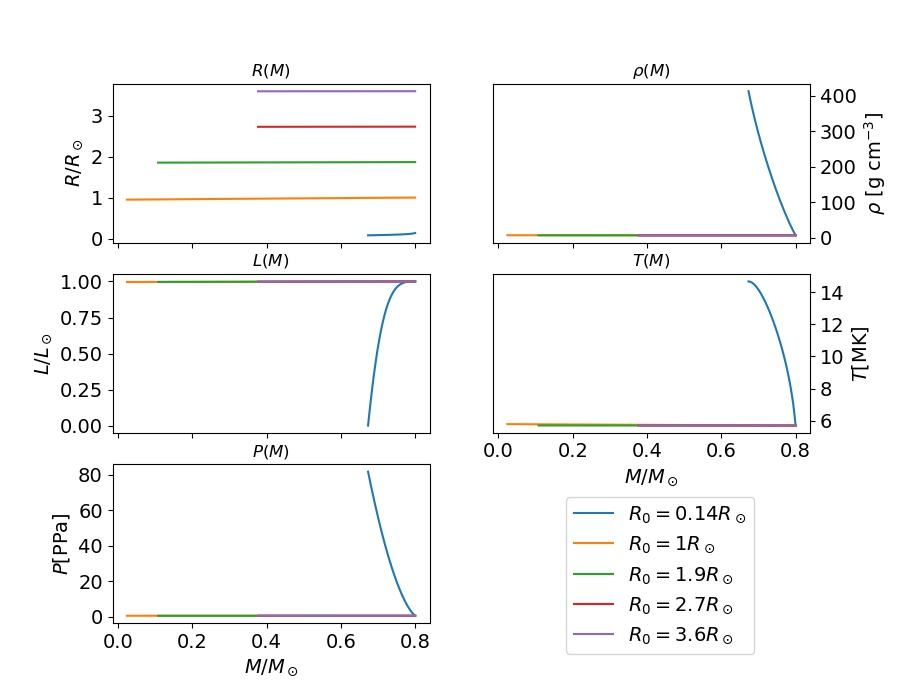
\includegraphics[width = \textwidth]{RadPlot.jpg}
		\caption{The plots show the radius $R$, density $\rho$, luminocity $L$, temperature $T$ and pressure $P$ for different initial radii. The color code indicates which graph har which initial condition.}
		\label{fig:rad}	
	\end{figure*}

	We found that running the simulations with a $\partial m$ found by variable step length with an error tolerance $p = 0.001$ gave a good balance between precision and run time. Thus the local relative error should be held bellow $10^{-3}$.
	
	When trying to test different radii, while holding other initial values constant and equal to the once provided, we got the plots shown in Fig. (\ref{fig:rad}). When looking at the plots we see that not much seems to change when using larger initial radii. But when using the lowest allowed initial radius $R_0 = 0.2\cdot0.72 R_\odot = 0.14 R_\odot$ was used, the changes to the different graphs were quite dramatic. The pressure, density and temperature skyrocketed, while the luminocity decreased dramatically, all within a mass change of about $0.2M_\odot$. This tells us that small radii seem to have a great effect on the outcome of the program. Specifically these changes appear to happen somwhere between $0.14-1R_\odot$. Since we ulimately want to find a solution where the luminocity and the radius both approach zero (within a 5\% tolerance of their tested initial values), an initial radius between $0.14-1R_\odot$ could be used in order to make the luminocity drop to zero.
	
	Next we iterated over different initial temperatures $T_0$ within the factor $\frac{1}{5}$ to 5 changes from the provided initial conditions, and produced the plots shown in Fig. ref{fig:temp}. In these plots the changes were generally a bit more subtle on avrage than when changing the initial radius. In this case we can observe that the higher initial temperatures do not seem to have that great of an effect on the outcome. All higher initial temperatures seem to have a similar behaviour. But when trying lower initial conditions, we see that the luminocity drops to zero quite quickly and almost linearly. Meanwhile the radius exhibit a similar behaviour, although it does not quite reach zero when the mass is zero. However it drops qite significantlly. The pressure, density and temperature behave quite similar in this case too, which is not a surpise considering they are tightly coupled through the equation of state. They all generally follow straight horisontal paths for all the higher initial temperatures. The lowest of the initial, however, cannot sustain such a high initial density, and drops fast in a matter of a short mass change, before settling into a more stable path. Also the lowest initial temperature makes the temperature graph increas quite fast about at the same place the density exhibits its initial drop. But generally the graph has a more increasing tendency compared to the other initial temperatures. Perhaps the most important fact to note for later, though, is that changing the initial temperature affects both how the radius and the luminocity look in a rather more significant way then changing the initial radius and density does. The latter two affecting the radius or the luminocity significantly but not the other one.
	\begin{figure*}
		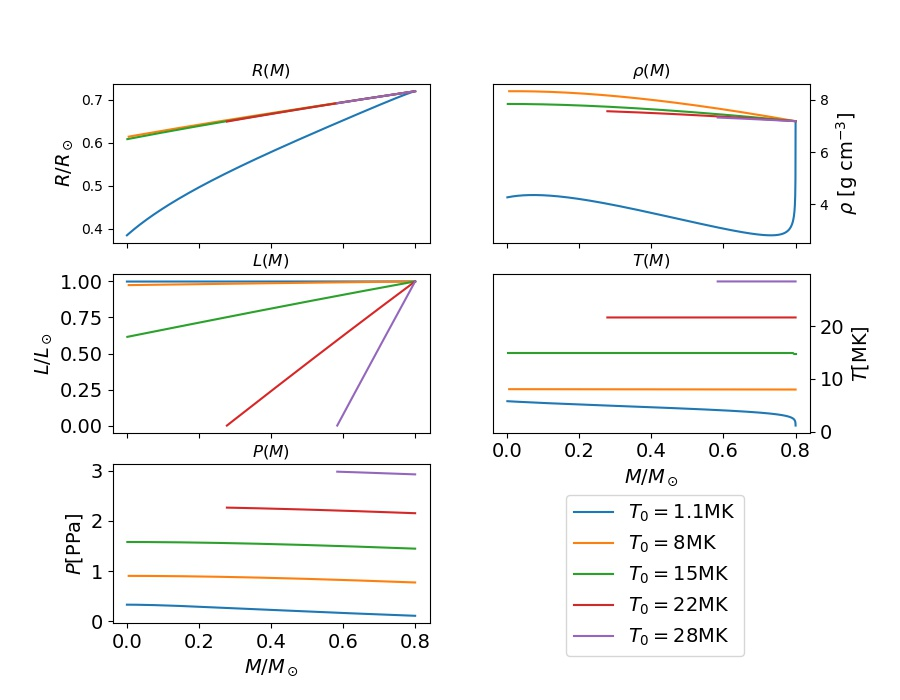
\includegraphics[width = \textwidth]{TempPlot.jpg}
		\caption{The plots show the radius $R$, density $\rho$, luminocity $L$, temperature $T$ and pressure $P$ for different initial temperatures. The color code indicates which graph har which initial condition.}
		\label{fig:temp}
	\end{figure*}
	Last the initial density was changes in a loop. The resulting plots can be seen in Fig. \ref{fig:rho}. In this case we see that the radius seems to have dropt quite a lot when reaching zero mass for a low initial density. The graph drops about $0.5R_\odot$ in total. The other initial densities do not affect the radius too much, as they only drop a little over the whole mass span in relatively linear fashion. In the luminocity plot the tendency is rather different. Here the lowest density changes the luminocity the least, but all over the luminocty is only changed by about 3\% of its initial value for the highest initial density. This makes sence since there is less material to fusion. In the plots showing the pressure and density, all the graphs show a simiilar behaviour. We see that again the higher initial values tend to behave the most like straight horisontal lines, while the lowest initial density results in a lightly more steap slope. The same tendency can be observed in the temperatures behaviour, where the higher initial densities result in more or less the same sightly increasing line like path. The lowest initial value, though, make the temperature increase about $2$ MK ove the whole mass span, compared to the roughly $1$MK change for the higher initial densities. Again it seems to be the lower initial values that exhibit the most interesting properties. Note that compared to the change of initial radius it is the luminocity that changes relatively little, while the radius as a function of mass decreases more significantlly.
	
	To sum up the knowlage achieved in the above mentioned changes in initial values; The change in initial radius made the luminocity drop to zero very fast, while leaving the radial distance as a function of mass relatively steady. The change in initial temperature changed both the temperature and the luminocity quite a lot, while changing the initial density made the radial distance change more, leaving the luminocity more or less unchanged.
	
	Thus when choosing the two initial value changes we want to iterate over in a double loop, as mentioned in the Method section, we choose the initial radius and density. That is because they made either the luminocity or radial distance change, but leaving the other alone. In theory we can thus change the luminocity to a satisfactory path, by changing the initial radius. While the initial density can be adjusted so that the radius also approaches zero when the mass does. The colorplots produced by this algorithm can be seen in Fig. \ref{fig:colorplot}. Clearly the same tendency previously observed is also seen in the colorplots. As seen in the luminocity plot in Fig. \ref{fig:colorplot}, luminocity tends towards zero for low initial radii, while the initial density does not have all to much of an effect. When looking at the radius plot in Fig. \ref{fig:colorplot} one can again observe that the low initial density makes the radial distance go towards zero, while the initial radius only has a relatively small effect. Last we can also see that the mass approaches zero for most initial radii and densities. Only the lowest intial radii make the mass not go to zero. In the combined plot in Fig. \ref{fig:colorplot} the sum of the three others is shown. One can clearly see a region of th colorplot where all three added plots go towards zero together, that is for low initial radius and density. In this region there are probabely several grid coordinates that would give a stabel star. 
	\begin{figure*}
		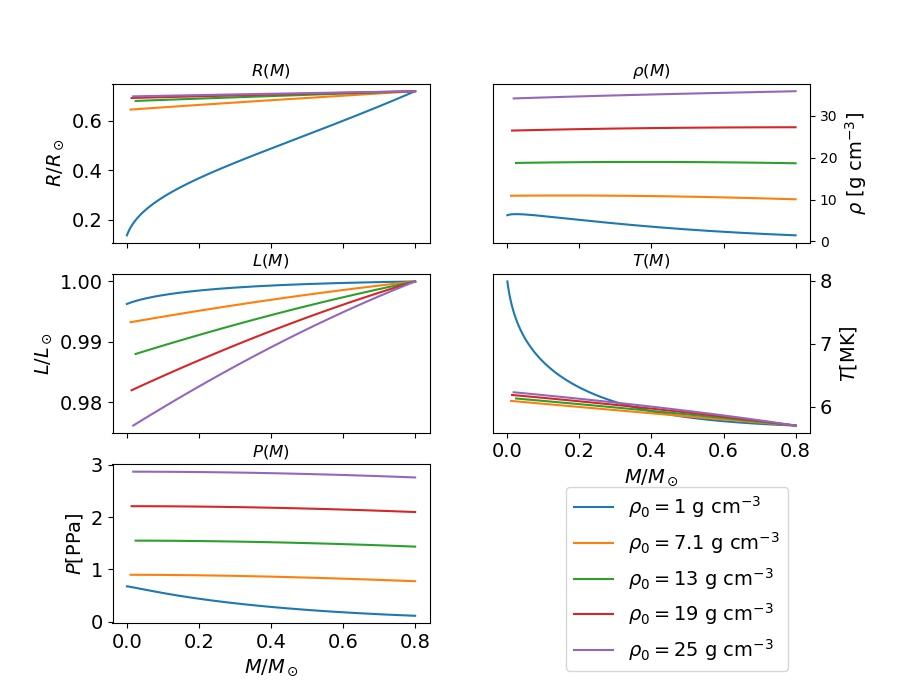
\includegraphics[width = \textwidth]{rhoPlot.jpg}
		\caption{The plots show the radius $R$, density $\rho$, luminocity $L$, temperature $T$ and pressure $P$ for different initial densities. The color code indicates which graph har which initial condition.}
		\label{fig:rho}
	\end{figure*}
	
	However the very best solution we were able to find was found by taking the minimum of the matrix of the function values in the combined plot. The minimum will thus be the solution which has the least deviation from the 5\% tolerance. Specifically we found the best initial value to be $R_0^\text{best} \approx 0.408 R_\odot$ and $\rho_0^\text{best} \approx 2.756$ g cm$^{-3}$ in addition to the other provided initial values. We found that for this model of a star the luminocity approached zero within 0.28\% of $L_\odot$, the radius approached zero within 0.73\% of the initial radius $R_0^\text{best}$ and the mass approached zero within 2.59\% of $M_\odot$. This means that all three quantities approach zero well within the 5\% tolerance, thus this can be considered a successfull model of a stellar radiation zone.
	
	Having found a good model of the stellar radiation zone we can take a look at how it lookes in detail across its cross section. In Fig. \ref{fig:beststar} one can see the mass $M(r)$, density $\rho(r)$, pressure $P(r)$, luminocity $L(r)$, temperature $T(r)$ and energy production $\epsilon(r)$ as functions of the radial distance $r$ from the stellar core of the best solution found. Yet again we see that the luminocity and mass approach zero closely when the radial distance does. The form of the density and pressure are as expected a close resemblance of eachother due to them being coupled by the equation of state. Also the temperature seems to follow the general tendency of the density and pressure, which is also to no surpise as it is part of the equation of state too. Generally it makes sence that the density and pressure go upwards when approaching the stellar core, because more and more matter pushes inwards from the outer layer the further the core is approached, making the pressure and density increase. Thus also the temperature seems to behave as it should, since a compressed gass tends to be warmed up. Thus since the ideal gas in this model are compressed more and more the further inwards we go, it is heated up more and more. When looking at the energy production $\epsilon(r)$ we see that its form also seems to resemble the pressure and density. This is also consistent with the theory, as the increasing density and temperature result in a higher probability of fusion reactions happening. That is because the higher density will result in a higher number of collisions between the atomic nuclei in the plasma. While the higher temperature results in the nuclei having a higher kinetic energy making it more likely that they can overcome the coloumb potential exerted by the atomic nuclei. 
	
	\begin{figure*}
		\includegraphics[width = \textwidth]{combined_contour.jpg}
		\caption{Each $R,\rho$-gridpoint in the three leftmost colorplots represent the last value of the luminocity $L_{last}/L_\odot$, radius $R_{last}/R_{init}$ and mass $m_{last}/M_\odot$ produced by solving the PDE system using the grid coordinates as initial radius and density. The rightmost plot represents the sum of the three other color plots.} 	
		\label{fig:colorplot}
	\end{figure*}
	
	\begin{figure*}
		\includegraphics[width=\textwidth]{BestStar.jpg}
		\caption{The figure shows the mass $M(r)$ (top left), density $\rho(r)$ (top right), pressure $P(r)$ (mid left), luminocity $L(r)$ (mid right), temperature $T(r)$ (low left) and energy production $\epsilon(r)$ (low right) as functions of the radial distance $r$ from the stellar core of the best solution to the PDEs found.}
		\label{fig:beststar}
	\end{figure*}
	\newpage
	\section*{Conclusion}
	To sum up we have made a program solving a coupled system of partial differential equations in order to make a model of the stellar radiation zone. By trying different initial value for radius, temperature and density at the outermost layer we got a feeling for how thay affect the simulations outcome. This knowledge was then used to formulate a systematic methode looping over a grid of initial radii and densitis to find the best initial values that produced a stabel stellar radiation zone. All in all the best model found seems to resemble a good model of a stellar radiation zone. It exerts all the behaviour one would expect across the cross section, were pressure, density, temperature and energy production all grow when travling inwards in the star. While the mass and luminocity droped to zero when reaching the centre of the star. Since the star seems to be well behaved we can conclude that we have found a stable solution of the stellar raiation zone.
	
	
	%\date{Received - / Accepted -}
	
	%\begin{figure}[t]
	%
	%\mbox{\epsfig{figure=filename.eps,width=\linewidth,clip=}}
	%
	%\caption{Description of figure -- explain all elements, but do not
	%draw conclusions here.}
	%\label{fig:figure_label}
	%\end{figure}
	
	
	\begin{acknowledgements}
		I thank my fellow student Bernhard Nornes Lotsberg for help and collaboration in this project.
	\end{acknowledgements}
\end{document}
